\chapter{Reinforcement Learning}
\label{ch:rl}
\thispagestyle{empty}

When we think about the nature of learning, the first thing that probably occurs to us is learning by examples, namely, learning from some interactions with the environment. Since we were children, we started interacting with the environment by taking actions and learning about the consequences of such actions in order to accomplish a goal (e.g. we start moving the feet and learn how to walk). 


Reinforcement Learning (RL) is a field of Machine Learning that closely resembles how living beings learn in nature. In this work we will explore the computational approach to learning from interaction, by considering a simplified yet powerful mathematical model. Reinforcement Learning is about learning what to do, how to map actions to each state, so as to maximize a reward signal. The learner is not told which actions to take, but rather he has to discover which actions are more valuable via trial and error. \\
This is not a trivial task, since actions can potentially have long-term effects. In fact, an action affects the next state, from where we can take another action that take us in another state and so on, substantially changing the rewards that we can take. Delayed rewards and trial and error search are the two most important aspects of reinforcement learning, that makes this problem both difficult and intriguing.

We will formalize the problem of reinforcement learning using a model taken from dynamical systems theory called Markov decision process. This model will be described in details in~\Cref{sec:mdp} but we will list here the basic principles behind this model. The main aspects that we want to capture are the interactions between an agent and the environment over time. A learning agent must be able to sense the state of its environment and take some actions, while the environment itself receives the actions from the agent and reacts by changing the state and giving feedbacks to the agent to complete the circle.
The agent must have a goal that relating to the state of the environment.\\
Markov decision processes are intended to include just these three aspects - sensation, action and goal - in their simplest possible forms without trivializing any of them.

One of the challenges that arise in reinforcement learning - opposed to other kinds of learning - is the trade-off between exploration and exploitation. To obtain a lot of reward, a reinforcement learning agent must prefer actions that it has tried in the past and found to be effective in producing reward. At the same time, though, discovering such actions requires a trial and error search. The agent has to exploit what it has already experienced in order to obtain reward, but it also has to explore in order to make better action selections in the future. This dilemma is that neither exploration not exploitation can be pursued exclusively without failing at the task: a fully exploit algorithm would likely choose sub-optimal actions while a fully exploratory behaviour will likely to take random actions without long-time awareness.\\
The agent must try a variety of actions and progressively favour those that appear to be the best. This dilemma can be made even harder when we consider stochastic rewards, where the agents must try the same actions multiple times to be sure about its estimated value. \\
The exploration-exploitation dilemma has been studied intensively for many decades, yet remains unsolved.



\section{Markov Decision Processes}
\label{sec:mdp}
In this section we will formalize the problem of reinforcement learning by defining a mathematical model called Markov decision process that will be used to model the interactions between the agent and the environment.
\begin{definition}
A Markov Decision Process (MDP) is a tuple $\left\langle \sspace, \aspace, \tfunc, \rfunc, \gamma, \mu \right\rangle$  where:
\begin{itemize}
\item $\sspace$ is the set of possible \textbf{states}
\item $\aspace$ is the set of possible \textbf{actions}
\item $\tfunc : \sspace \times \aspace \rightarrow \Delta (\sspace)$ is the \textbf{transition function} that, given the current state and current action, outputs a probability distribution over the next state.
\item $\rfunc : \sspace \times \aspace \rightarrow \mathbb{R}$ is the \textbf{reward function} that maps a scalar reward to every state-action pair
\item $\gamma$ is the \textbf{discount factor}
\item $\mu : \Delta ( \sspace )$ is a probability distribution over the \textbf{initial state}. 
\end{itemize}
\end{definition}

This mathematical model is very general and can be used to model different problems:

\begin{example}[Chess]
The game of chess can be modelled as an MDP with a discrete state space that encodes the position of all the pieces in the checkerboard, a discrete action space encoding all the possible moves of the pieces, deterministic transition function that follows the rules of the game and a possible reward function:
\begin{equation*}
\rfunc(s,a) = \begin{cases}\,\,\,\,\,1 & \textrm{Player wins} \\ -1 & \textrm{Player does not win} \end{cases}
\end{equation*}
\end{example}

\renewcommand\windowpagestuff{\centering 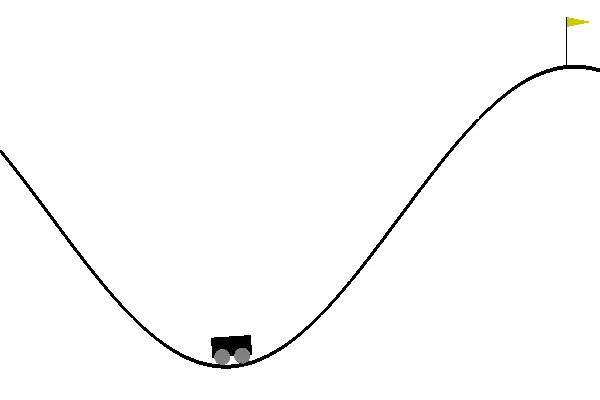
\includegraphics[width=5.5cm]{pictures/mountain_car.jpg} \captionof{figure}{Mountain car task}}
\opencutright

\begin{adjustbox}{valign=C,vspace=0bp,minipage={1.0\linewidth}}
\begin{example}[Mountain Car]
\begin{cutout}{0}{7.5cm}{0pt}{12}
A car is placed between two hills and can move left or right. The goal is to reach the top of the right hill, but the engine is not powerful enough to directly climb the hill, so the optimal solution is to gain velocity by first going in the opposite direction. This task can be modelled with a continuous state space $\sspace \in [-2, 2]$, continuous action representing the force applied to the car $\aspace \in [-1, 1]$, deterministic transition function given by physics laws and the following reward function:
\end{cutout}

\begin{equation*}
\rfunc(s,a) = \begin{cases} +100 & \textrm{when } s \geq 1.5 \\ -a^2 & \textrm{otherwise} \end{cases}
\end{equation*}

This problem is particularly difficult for its exploration need: the agent, in fact, must explore very much in order to see the goal, but this comes with a cost associated to the square of the taken action.
\end{example}

\end{adjustbox}


\renewcommand\windowpagestuff{\centering 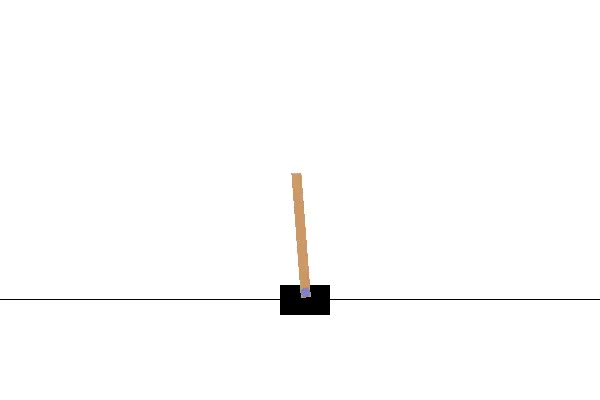
\includegraphics[width=5.5cm]{pictures/cartpole.jpg} \captionof{figure}{Cartpole task}}
\opencutleft
\begin{adjustbox}{valign=C,vspace=0bp,minipage={1.0\linewidth}}
\begin{example}[Cartpole]

\begin{cutout}{3}{0pt}{8cm}{13}
A pole is attached to a cart by a joint that is free to rotate. The cart moves along a frictionless track either left or right. The pole starts upright, and the goal is to prevent it from falling over by moving the cart left-right.\\
This task can be modelled with a continuous multidimensional state space $\sspace \in \mathbb{R}^4$. The state features are: the position of the cart $s_0 \in [-2.4, 2.4]$, its velocity $s_1 \in [-\infty, \infty]$, the pole angle $s_2 \in [-\frac{\pi}{2}, \frac{\pi}{2}]$ and its angular velocity $s_3 \in [-\infty, \infty]$. The action space is continuous $\aspace \in [-1, 1]$ and represents the force to be applied on the cart. The transition function is given by physics laws and the reward is $+1$ for every step until the episode ends. An episode ends when a maximum step limit $H$ is reached or when the pole is inclined more than 15 degrees from vertical.


\end{cutout}

\end{example}
\end{adjustbox}

An agent in a MDP starts from an initial state drawn from the probability distribution $\mu$, $s_0 \sim \mu$. From this state, the agent can interact with the environment by applying an action $a_0 \in \aspace$. The environment receives action $a_0$ and reacts to this stimulus by returning to the agent the next state $s_1$ drawn from the transition function $s_1 \sim \tfunc(s_0, a_0)$ and a scaler reward $r_1 = \rfunc(s_0, a_0)$. From its new observation, the agent can continue the interaction with the environment by choosing another action $a_1$ and so on until it reaches the goal. We define the collected sequence of states, actions and rewards $\tau \sim s_0, a_0, s_1, r_1, a_1, s_2, \ldots$ trajectory. Sometimes we will refer to a trajectory with terms like samples or experience, since these collected informations will be used for the learning procedure.


Intuitively, the agent aims at maximizing the sum of the collected rewards. However this naive sum of rewards do not apply if we consider infinite-horizon MDPs, which is a common setting in the literature. In fact, summing over potentially infinite-length trajectories will cause the cumulative reward to grow indefinitely and lose its original meaning. (e.g. earning +1 at every step will have the same meaning of earning +100 at every step, since over an infinite horizon they will both grow to infinity).\\
For this reason, it is common to consider a generalized version where we apply a discount factor $\gamma$ to the immediate reward and consider the cumulative discounted reward:
\begin{definition}[Cumulative discounted reward]
\begin{equation*}
R = \sum_{t=0}^{\infty} \gamma^t r_t
\end{equation*}
where $\gamma \in [0,1]$ is called discount factor. 
\end{definition}
Note that the naive cumulative reward can be used by setting $\gamma=1$, and this is commonly used when the horizon is finite. 

However, the addition of the discount factor has a well-known two-fold meaning: at a first glance, it represents how the agent is interested in future rewards. With $\gamma$ close to $0$, we have a myopic behaviour, where we are only interested in immediate rewards rather than long-term investments. With $\gamma$ close to $1$, instead, we are giving more value to long-term rewards. In the second place, $\gamma$ can also represent the probability that the simulation will continue for one more step. If $\gamma$ is low, we should strive to get as much as we can because we don't have any assurance that we could last one more step.
The discount factor usually depends on the domain and the goal that we want to achieve: a long-term goal will require a value of $\gamma$ close to $1$.


The actual value of the discounted cumulative reward depends on the interaction of the agent over a trajectory. Many factors come into play to influence this objective function, most importantly the behaviour of the agent (e.g. which actions the agent chooses). The way an agent interacts with the environment and hence characterizes its behaviour is defined by the policy function:
\begin{definition}
A policy $\pi: \sspace \rightarrow \Delta (\aspace)$ is a function that for each state $s \in \sspace$ outputs a probability distribution over the actions in $\aspace$. In other words, from state $s$ the agent will choose action $a$ with probability $\pi(a \mid s)$.
\end{definition}

The policy is one of the main ingredients of reinforcement learning, as it is the final result of a reinforcement learning algorithm. The policy tells the agent which actions to choose.
Starting from an initial state $s_0$, the agent will choose action $a_0 \sim \pi(\cdot | s_0)$ drawn from the action distribution induced by the policy in this state. We can see that a policy completely define all the interaction with the environment, hence we can define its performance or expected return in this way:
\begin{definition}[Performance of a policy $\pi$]
The performance (or expected return) of a policy $\pi$ under initial state distribution $\mu$ is:
\[
J_\mu(\pi) = \EV[a_k \sim \pi, s_0 \sim \mu]{R}
\]
that is, the expected value of the discounted cumulative reward obtained by following the policy $\pi$ starting from an initial state drawn from $\mu$.
\end{definition}
Having defined this new metric, we can easily rank each policy according to its performance: a policy $\pi_1$ is better than a policy $\pi_0$ if $J_\mu(\pi_1) > J_\mu(\pi_0)$. The next step will be to find the policy that scores the highest performance for a given MDP. This is the goal of solving an MDP.

\textbf{Problem formulation:}\quad
To solve a MDP means to find an optimal policy $\pi^*$ that maximizes the average cumulative reward. More formally we want to find $\pi^*$ such that $J_\mu(\pi^*)=\EV[a_k \sim \pi^*, s_0 \sim \mu]{R}$ is maximum.

To recap, we can define the interaction between an agent and the environment as a sequence of state-action-reward tuples called trajectory. The environment is modelled with a markovian transition function - a function that takes the current state-action pair and outputs a probability distribution over the next state. The Markov property assures that the transition function depends only on the current state and not on the entire history of the interaction. The agent receives a reward for every action it takes and aims at maximizing the discounted cumulative reward. The behaviour of the agent is characterized by the policy function $\pi$, which yields for every state $s$ a probability distribution over the actions $\pi(a|s)$. Every policy can be ranked by its performance or expected reward obtained following the policy from an initial state drawn from $\mu$. A MDP is considered solved when we find an optimal policy $\pi^*$ whose performance value is maximal.

Here we define a new quantity that will be useful later which is the discounted future state distribution. This function calculates the visitation frequency for each state $s\in\sspace$ by starting from $s_0\sim\mu$ and following policy $\pi$. This quantity is defined as follows:
\begin{definition}[Future state distribution]
The (discounted) future state distribution is defined as: 
\[
d_{\mu}^{\pi}(s) = (1-\gamma)\sum_{t=0}^{\infty} \gamma^t Pr(s_t = s)
\]
This quantity identifies the expected state distribution starting from $s_0 \sim \mu$ and following policy $\pi$. 
\end{definition}

Following this definition, we can reformulate the performance of a policy $\pi$ as a function of the state distribution $d_\mu^\pi(s)$.

\begin{definition}[Performance given state distribution]
The performance of a policy $\pi$ given an initial state distribution $\mu$ can be expressed as: 
\begin{equation*}
J_{\mu}(\pi) = \int_{\sspace} d_{\mu}^{\pi}(s) \int_{\aspace} \pi(a \mid s) \rfunc(s,a) \de a \de s
\end{equation*}
\end{definition}


\subsection{Value functions}
So far we have defined what is a MDP and what does it mean to find an optimal policy $\pi*$. In this part we will take the problem under a different perspective by considering the value of each state. The value of a state should not consider only immediate rewards, but should also consider the discounted sum of all the rewards that the agent may get. This idea of including delayed rewards to describe the value of a state is defined by the state-value function:

\begin{definition}[State-value function]
The value of a state $s$ that can be obtained by running policy $\pi$ is given by:
\[
V^{\pi}(s) = \int_{\aspace} \pi(a \mid s) \left( \rfunc(s,a) + \gamma \int_{\sspace} \tfunc(s' \mid s, a) V^{\pi} (s') \de s' \right) \de a
\]
\end{definition}

The state-value function $V^\pi(s)$ encodes the average reward that we will obtain starting from state $s$ and following $\pi$ thereafter. Note that this is a recursive definition as to compute the value of state $s$ we need to compute the values of all the states reachable from $s$ and so on. This definition allows us to give a different way to calculate the performance of a policy based on the value function and initial state distribution
\[
J_\mu(\pi) = \int_{\sspace}\mu(s)V^\pi(s)\de s
\]
The value of the optimal policy $\pi^*$ is called optimal state-value function $V^*(s) = V^{\pi^*}(s)$. The optimal value function is unique, even if multiple optimal policies may exist. We can restate the goal of an RL algorithm as a maximization over the policy space of the state-value function for all states:
\[
\pi^* = \arg\max_{\pi \in \Pi} V^\pi(s),\qquad \forall s \in \sspace
\]
The value function is useful to consider to solve a MDP, however it does not say anything about the actions that brought to that value. Since our main goal is to find an optimal policy, we need a way to assign a value also to the actions. The following statement will define the action-value function:

\begin{definition}[Action-value function]
The action-value function for a policy $\pi$ is defined as follows:
\[
Q^{\pi}(s, a) = \rfunc(s, a) + \gamma \int_{\sspace} \tfunc (s' \mid s, a) \int_{\aspace} \pi(a' \mid s') Q^{\pi} (s', a') \de a' \de s'
\]
\end{definition}

The action-value function defines the value that we can obtain starting from state $s$ and executing action $a$. This function encodes more informations since we can retrieve the state-value function by averaging the action-value function over all actions: $V^\pi(s) = \EV[a\in\aspace]{Q^\pi(s,a)}$. \\
Similarly to the definition of the optimal value function, the optimal action-value function $Q^*$ is defined to be the action-value function of the optimal policy $Q^*(s) = Q^{\pi^*}$. 

The action-value function let us introduce another quantity of particular interest for the algorithms described in \Cref{sec:solve-mdp} called the advantage function. The advantage of action $a$ over policy $\pi$ encodes how much we can gain by performing action $a$ instead of following the policy $\pi$ and is defined as follows:
\begin{definition}[Advantage function]
The advantage function of action $a$ over policy $\pi$ is defined as:
\[
A^{\pi}(s,a) = Q^{\pi}(s,a) - V^{\pi}(s)
\]
\end{definition}

The advantage function can also be used to compare two policies $\pi'$ and $\pi$: for every state $s$ we compute the advantage of selecting an action from $\pi'$ rather than $\pi$. In this case it is called policy advantage function.
\begin{definition}[Policy advantage function]
The advantage of policy $\pi'$ with respect to policy $\pi$ in state $s$ can be computed as:
\[
A_\pi^{\pi'}(s) = \int_{\aspace} \pi'(a|s)A^\pi(s, a) \de a
\]
whose expected value over the states is called expected policy advantage function:
\[
\poladv[\pi,\mu][\pi'] = \int_{\sspace} d_\mu^{\pi}(s)A_\pi^{\pi'}(s) \de s
\]
\end{definition}


Note that the greedy policy is the one that has always non-positive advantage for each state. 


Bellman optimality operators

Put algorithms and figures

\section{General methods to solve a MDP}
\label{sec:solve-mdp}
A MDP can be solved in various ways. We have seen in the previous section that a MDP is solved when we find an optimal policy $\pi^*$ that generates the optimal value function $V^*(s)$. However, a learning procedure can be classified in several classes:
\begin{itemize}
\item On-policy: the behaviour policy corresponds to the target policy. This means that every collected trajectory is sampled from the current policy.
\item Off-policy: the target policy differs from the behaviour policy. This happens when we are trying to learn from samples that are drawn from a policy that is different from the current policy.
\end{itemize}

Another difference between the learning algorithms arises when we consider the amount of informations that we know during learning:
\begin{itemize}
\item Model-based RL algorithms have an exact information about the MDP. This means that the learning agent knows exactly the transition function $\tfunc$, and the reward function $\rfunc$. This is the easiest scenario because the MDP can be solved even without taking any sample from the actual system.
\item Model-free RL algorithms, instead, have no information about the model, which is learned by collecting samples from the actual system.
\end{itemize}

From now on, we will focus only on model-free algorithms that learns on-policy. This is the typical setting for robotic control, since we don't have the possibility to explicitly model the environment and we can test our policy directly on the system.

The next sections will describe the three main methods that are used to solve a MDP: policy iteration, value iteration and policy seach.

\subsection{Policy iteration}
Policy iteration algorithms aims at finding a sequence of policies $\pi^0, \pi^1, \ldots$ such that the sequence of the corresponding value functions $V^{\pi^0}, V^{\pi^1}, \ldots$ is non-decreasing. 
This can be achieved by splitting each iteration in two phases:
\begin{itemize}
\item Policy evaluation: we evaluate the current policy $\pi^k$ on the MDP and we estimate the corresponding action-value function $Q^{\pi^k}$.
\item Policy improvement: we improve the current policy $\pi^{k+1} \gets \pi^{k}$ based on the action-value function $Q^{\pi^k}$.
\end{itemize}

The policy improvement step selects the greedy policy:
\begin{equation}
\pi^{k+1}(s) \in \arg \max_{a \in \aspace} Q^{\pi^k}(s, a)  
\end{equation}

It is guaranteed that $V^{\pi^k+1} \geq V^{\pi^k}$ directly from the definition of greedy policy. Moreover, this algorithm is guaranteed to converge to the optimal policy $\pi^*$ when the state-action function $Q(s,a)$ can be computed exactly.

The limitations of this approach are at least two:
\begin{itemize}
\item In practical scenarios it is not possible to exactly evaluate the action-value function due to the stochasticity of the environment and the sampling nature of the algorithm.
\item This method can only be applied to discrete MDP, that is MDPs where both $\sspace$ and $\aspace$ are discrete sets. This is typically not the case for robotic control, where the state and action pair is typically continuous.
\end{itemize}


The value function can be used to define an ordering between policies:
\begin{definition}[Policy improvement]
Given two policies $\pi, \pi' \in \Pi$, policy $\pi'$ is better than or equal to ($\succcurlyeq$) policy $\pi$ when the value function of $\pi'$ is greater than or equal to the value function of $\pi$ in all states:
\[
\pi' \succcurlyeq \pi \Longleftrightarrow V^{\pi'}(s) \geq V^{\pi}(s),\quad \forall s \in \sspace
\]
\end{definition}

The following theorem will state that the optimal policy will correspond to the maximal of the ordering relation (i.e the element that is better than or equal to all other policies):

\begin{theorem} 
For any MDP the following statements hold:
\begin{itemize}
\item there exists an optimal policy $\pi^* \in \Pi$ such that $\pi^* \succcurlyeq  \pi$, $\forall \pi \in \Pi$.
\item all optimal policies $\pi^*$ have the same optimal value function $V^{\pi^*}(s) = V^*(s) \forall s \in \sspace$ .
\item there always exists an optimal policy $\pi*$ that is deterministic.
\end{itemize}
\end{theorem}

This is an important result since we can develop an iterative algorithm that can automatically find the optimal policy. In fact, starting from any policy $\pi$, we can identify a policy $\pi' \succcurlyeq \pi$ that improves the current policy until we find the optimal policy $\pi^*$. This method is called policy iteration, and it is proven to converge in a finite number of steps. Although this method is general, we still have to find a policy $\pi' \succcurlyeq\pi$. A common choice for $\pi'$ is the greedy policy $\tilde{\pi}$. The greedy policy is a policy that maximizes the action-value function for each state:
\[
\tilde{\pi}(a|s) = \arg\max_{a\in\aspace} Q^{\pi}(s,a)
\]




\subsection{Value iteration}
Value iteration algorithms 

\subsection{Policy search}

\section{Policy gradient methods}
\subsection{Gradient estimation}
\subsection{Policy gradient theorem and G(PO)MDP}
\subsection{Baselines}
\subsection{Actor critic}



 